\documentclass[twoside,privacy]{textmf-local/srathesis}
% options:
% [earlydraft] - Settings for quick draft printouts
% [germanthesis] - Thesis is written in German
% [plainunnumbered] - Don't print numbers on plain pages
% [privacy] - Generate a more privacy aware PDF (exclude birthplace and birthday)
% [twoside] - double sided
% [watermark] - Print current time/date at bottom of each page

% You can use dataref to reference data points from your experiments symbolical.
% Thereby, you are able to redo experiments, without reinserting and recalculating all numbers.
\usepackage{dataref}
\usepackage{pgfplots}
\renewcommand{\baselinestretch}{1.25}
\usepackage{xcolor}
\usepackage{tcolorbox}
\usepackage{multicol}
\definecolor{ba-green}{HTML}{008000}
\definecolor{ba-red}{HTML}{dc143c}

\definecolor{light-gray}{gray}{0.95}
\newcommand{\code}[1]{\colorbox{light-gray}{\texttt{#1}}}
% \input{data/dref}

\bibliography{references}
% The OSG also has a central bibliography that we share with the System- and Rechnerarchitecture (SRA) group from Hannover.
%\bibliography{bib/sra-ext}
%\bibliography{bib/sra-own}
%\bibliography{bib/osg-own}

\author{Elias Frank}
\title{A field study using ReUpNix as a host for Microsoft's Azure IoT Edge platform}
\thesistype{Bachelorarbeit im Informatik}
\thesiscite{Bachelor's Thesis}
\birthday{15. Juni 1999}
\birthplace{Hamburg}
\thesisstart{tbd}
\thesisend{tbd}
\examiner{Prof. Dr.-Ing. Christian Dietrich}
\coexaminer{XXX}
\advisors{& \textbf{Niklas Gollenstede (M.Sc.)}\\
          & \textbf{}}

\begin{document}

\pagestyle{fancy}
\pagenumbering{roman}

\maketitle

\addcontentsline{toc}{chapter}{Abstract}
\begin{otherlanguage*}{american}

The growth of the \ac{IoT} in industries like production, manufacturing, and
agriculture has led to a wide range of innovations and new products. Currently,
all major cloud providers such as Microsoft, Google, Amazon's AWS, and IBM offer
\ac{IoT} services and solutions to their customers. However, many \ac{IIoT} devices,
which are installed in remote locations, such as offshore oil rigs or airplanes,
have limited, unstable, or costly network connections. Techniques to
minimize the \ac{IIoT} software's network traffic both in message size
(such as \textit{ProtoBuf} encoding or compression), and in message amount
(such as local processing with edge computing) have already been established.
However, the image size, update, and consistency of the underlying operating
system is still a challenge. With Microsoft's \textit{Azure IoT Device
Update} service, for example, the entire image for the operating system is sent
to the device and then written to a secondary partition. This results in hundreds
of megabytes being transmitted.

In this study, it was investigated if the \textit{NixOS}-based \textit{ReUpNix}
can be used as a suitable host operating system for Microsoft's commercial
\ac{IoT} platform \textit{Azure IoT Edge}, since its image size is significantly
smaller than Microsoft's recommended Linux images.
The  minimum set of components and features that have to be added to heavily
minified \textit{ReUpNix} have been identified in order to have the required
functionality for the
Docker-container-based \textit{Azure IoT Edge}, while remaining at a small
footprint in disk size.

With \textit{ReUpNix} as a host operating system for \textit{Azure IoT Edge}, a
43\% smaller image size due to the minification was observed and 90\% smaller size of
system updates due to the fact that only differences are sent, compared to
Microsoft's recommended \textit{Ubuntu 22.04} image.
Further, it was shown that it is possible to install Docker container
layers on the device, such that the amount of data that needs to be transmitted
in the case of a container update with \textit{Azure IoT Edge} is reduced, if
an efficient compression is used.
However, \textit{NixOS}-based systems do not receive official support from
Microsoft and product managers need to decide if the benefits outweigh the loss
of Microsoft's support.

\end{otherlanguage*}


\chapter*{Kurzfassung}
\addcontentsline{toc}{chapter}{Kurzfassung}
\begin{otherlanguage*}{ngerman}
Das Wachstum des Internet of Things (IoT) in Branchen wie Produktion, Fertigung
und Landwirtschaft hat zu einer Vielzahl von Innovationen und neuen Produkten geführt.
Derzeit bieten alle großen Cloud-Anbieter wie Microsoft, Google, Amazons AWS und IBM
ihren Kunden IoT-Dienste und Lösungen an.
Allerdings gibt es einige industrielle IoT-Geräte (IIoT), welche
 an abgelegenen Orten installiert sind, wie z. B. auf Bohrinseln oder in Flugzeugen,
die begrenzte, instabile oder teure Netzwerkverbindungen haben.
Methodiken zur Minimierung des Netzwerkverkehrs von IIoT-Software sowohl in der
Nachrichtengröße (wie ProtoBuf oder  Kompression) als auch in der Anzahl der Nachrichten
(z. B. lokale Verarbeitung mit Edge Computing) wurden bereits etabliert.
Allerdings bleiben die Größe, das Update und die Konsistenz des zugrunde liegenden
Betriebssystems eine Herausforderung. Mit Microsofts Azure IoT Device Update Service
wird beispielsweise das gesamte Image für das Betriebssystem an das Gerät gesendet
und dort auf eine sekundäre Partition geschrieben. Dies führt zu hunderten von Megabytes
die übertragen werden.

In dieser Studie untersuchen wir, ob das NixOS-basierte ReUpNix als geeignetes
Betriebssystem für Microsofts kommerzielle IoT-Plattform
IoT Edge genutzt werden kann, da das Betriebssystem signifikant kleiner ist als Microsofts empfohlenes
Betriebssystem Ubuntu 22.04. Dafür haben wir die minimalen Komponenten und Funktionen,
die zum stark minimierten ReUpNix hinzugefügt werden müssen, identifiziert, um die
Docker-Container-basierte Azure IoT Edge Runtime zu unterstützen, während wir
weiterhin einen kleinen Fußabdruck auf der Festplatte beibehalten.

Mit ReUpNix als Host-Betriebssystem für Azure IoT Edge haben wir eine 43\%
kleinere Imagegröße aufgrund der Minimierung und 90\% kleinere Größe von
Updates, die gesendet werden müssen, da nur die Unterschiede in den Dateien gesendet
werden, im Vergleich zu Microsofts empfohlenem Ubuntu 22.04 Image. Weiterhin haben
wir gezeigt, dass es möglich ist, Docker-Container-Layer auf dem Gerät zu installieren,
so dass die Menge an Daten, die im Falle eines Container-Updates mit Azure IoT Edge
übertragen werden muss, reduziert wird, sofern man effizientere Kompression verwendet.
 Allerdings erhalten NixOS-basierte
Betriebssysteme keine offizielle Gewährleistung von Microsoft und Produktmanager
müssen entscheiden, ob die Vorteile den Verlust der Gewährleistung von Microsoft überwiegen.

\end{otherlanguage*}

\acresetall

\cleardoublepage
\tableofcontents

\cleardoublepage
\pagenumbering{arabic}

% \section{Context}
Since its first mention in 2006 \cite{Adelmann2006ToolkitFB} the \ac{IoT}
is a growing industry sector and active research field. A 2018 study conducted
by Dachyar et al., showed that \ac{IoT} has been continuously growing, is expected
to grow further, and will rise in demand for research and commercial application
because of its function to connect a variety of devices. The primary industries
where \ac{IoT} devices and applications are used today are manufacturing,
agriculture, public service, electronics, health, energy, and mining.
While most research is focused on topics such as security, protocols, energy and
power consumption \cite{dachyar2019knowledge}.

\ac{IoT} devices that are deployed in the mining and energy industry are often
installed in locations with limited, unreliable, or expensive network
connectivity, such as off-shore oil rigs or underground mining sites.
Some other industries have similar challenging installation sites, such as
satellites \cite{electronics8111247}, cargo ships \cite{9090272}, and remote weather stations \cite{info12040146}.
The limited bandwidth available in these remote locations poses a significant
obstacle for transmitting large amounts of data reliably and efficiently,
requiring innovative solutions for data optimization.

To address these challenges, there are already several approaches to compress
the transmitted data without a loss of information, which have shown to reduce
the data transmitted but also require more computing power on the \ac{IoT}
devices \cite{9243457}. An additional technique to reduce the amount of data
is to use a more efficient serialization format, such as Google's \textit{ProtoBuf}
which has shown to reduce the size of data transmitted for a particular application
by 83\% and 80\% in comparison to \textit{JSON} and \textit{BSON} respectively \cite{7765670}.
Lastly, when switching to an edge computing approach, the data can be preprocessed
and aggregated before sending it to the cloud, which reduces the amount of data
transmitted.


\section{Problem}
As applications often gain functionality and complexity with each release, the
size of software may also increase. For \ac{IoT} devices operating in environments
with limited bandwidth, this is an increased challenges. One case where this is
particularly evident is the \textit{Linux} kernel used by many \ac{IoT} and embedded
devices, which has expanded in size with every new release \cite{linux-kernel-report}.

However, product managers and developers are advised to update their devices with
the latest software, since
research has shown that updating security issues in \ac{IoT} systems as quickly
and as frequently as possible significantly enhances the security of these systems.
This is especially important for \ac{IIoT} devices, which have an extended attack
surface and where an outage can impose physical and financial damage \cite{s20247160}.
For \ac{IoT} devices with limited connectivity, crucial security updates can be
significantly delayed or even impossible to apply, as the update size may exceed
the available bandwidth or disk storage. But not just the security of \ac{IoT}
devices is improved by frequent updating. Anand et al. showed in 2018 that the
performance and reliability of \ac{IoT} applications can be significantly improved
by updating frequently \cite{Anand2018}.

When updating the \ac{OS} for an \ac{IoT} device it is very common to use an
A/B partition scheme, which will keep the device operational while downloading
and installing the latest version to the inactive partition and then switch with
a reboot once the update is complete. However, this approach is impractical for
devices which have limited storage, as the inactive partition will consume
half of the available storage. Further and most importantly, when updating,
it is required to download an entire bootable \ac{OS} image which can be
hundreds of \ac{MB} in size. This is not feasible for devices with limited
internet connection.

For \ac{IoT} applications that are using an edge computing architecture, the popular
approach is to use \ac{OCI}-containers (e.g. Docker) to package and update applications.
However, a large scale study conducted by Zhao et al. showed that 80\% of the
70,000 most popular \ac{OCI}-container images on \textit{Dockerhub} are more than
190 \ac{MB} in size, and contain a high amount of duplicate files shared across the images
and layers, especially for the images which are larger than 190 \ac{MB} \cite{9242268}.
This has the serious implications that updating \ac{OCI}-container images with
the existing methodology on a device with limited bandwidth is also impractical
and challenging.
\clearpage

\section{Strategy}
To address the problem of reliably updating \ac{IoT} and \ac{IIoT}
devices with limited bandwidth, it needs to be investigated if using a different
update strategy in contrast to A/B partitioning can reduce the amount of data transmitted.
It has been selected \textit{reUpNix} as the operating system to investigate, as its
update mechanism is specifically designed for \ac{IoT} and embedded devices with
limited bandwidth and storage \cite{gollenstede:23:lctes}. However, an integration
with a popular \ac{IoT} platform cloud services and \textit{reUpNix} has not
been done yet. The \textit{NixOS}-based \textit{reUpNix} provides a reproducible
build system, which is highly desirable property for keeping a consistent state
in a large fleet of \ac{IoT} or \ac{IIoT} devices.

As a cloud platform for \ac{IoT}, Microsoft's \textit{Azure IoT} has been chosen
as it is one of the most popular cloud platforms for \ac{IoT} and \ac{IIoT} applications.
\textit{Azure IoT Edge} in particular extends \textit{Azure IoT} to run
\ac{OCI}-containers on \ac{IoT} devices, which is a popular approach for edge
computing.

In section \ref{sec:update-size} a strategy has been designed to update the \ac{OS} of \ac{IoT} device running
\textit{Azure IoT Edge} using \textit{Azure IoT Device Update Service} with
\textit{reUpNix}'s update mechanism. The strategy needs to reduce the transmitted data
for an update significantly in comparison to using a full \ac{OS} image in an
A/B partition schema. Additionally, it needs to be verified that using a different
\ac{OS} than the one recommended by Microsoft does not significantly impact
the reliability and performance of the \ac{IoT} device.


Not just the \ac{OS} needs to be updated but also the \ac{IoT} applications
running as \ac{OCI}-containers on the device. To achieve this, 
a strategy in section \ref{sec:container-updates} has to be proposed,
using \textit{reUpNix}'s \ac{OS} update mechanism to reduce the transmitted data
size in comparison to using \code{docker pull}. The proposed strategy must
reliably save bandwidth for the popular \ac{OCI}-container images from
\textit{Dockerhub} while also not significantly increasing the disk storage
requirements on the device and integrating well with the existing container
runtime and \textit{Azure IoT Edge}.



\chapter{Fundamentals}
\label{sec:fundamentals}
This chapter introduces the major concepts, technologies,
and software relevant to this thesis. First, it will introduce the operating
systems \textit{Ubuntu 22.04}, \textit{Yocto Kirkstone Linux}, \textit{NixOS},
and \textit{ReUpNix}, which we will use for comparison in the later experiments.
Further, we will introduce the \textit{Azure IoT Edge} platform by Microsoft,
with all the components that were used.
Finally, the last sections will give an overview about the related work.

\section{Technology}
\subsection{Ubuntu 22.04}
\textit{Ubuntu 22.04} is the latest long term support release of the
\textit{Linux}-based operating system \textit{Ubuntu} developed by Canonical.
It will receive updates and support for the next 5 years, until April
2027 \cite{ubuntu-releasenote}. Additionally it is also one of Microsoft's
recommended operating systems to run containerized applications with
\textit{Azure IoT Edge} on Linux \cite{msdoc-supportetplatforms}.

\subsection{Yocto Kirkstone Linux}
The \textit{Yocto Project} is an open-source collaboration project that provides tools
and resources for building custom Linux-based systems for embedded devices.
\textit{Yocto Kirkstone Linux} is a recent long-term support release of the
\textit{Yocto Project}, which will receive support until April 2026 \cite{yocto-releases}.

\subsection{NixOS}
\textit{NixOS} is a \textit{Linux}-based operating system that uses the purely
functional package manager \textit{Nix}. It is currently maintained as
an open source project by the non-profit organization \textit{NixOS Foundation}
and the \textit{NixOS Community}. The project started in 2003 by Eelco Dolstra,
who is the current president of the \textit{NixOS Foundation}, as
a research project at the Utrecht University \cite{dolstra2003} and was introduced
as \textit{NixOS} in his 2008 paper "NixOS: A Purely Functional Linux Distribution".

A \textit{NixOS} system is configured with a set of configuration files, which
are evaluated by the \textit{Nix} package manager to produce a complete system.
The configuration files are written in the functional \textit{Nix} programming language,
which has the advantage of being declarative and reproducible. Further, \textit{Nix}
utilizes cryptographic hashes to verify the integrity of the inputs and outputs
for any given build. This means that the same configuration inputs produce the
same system. This approach aims to improve the correctness and reliability of
system deployments over traditional system build tools \cite{dolstra2006}.

A key concept of \textit{NixOS} is the \textit{Nix Store}, where all packages,
files, configurations, and other artifacts that the system requires are stored.
The \textit{Nix Store} is a immutable directory tree, where every \textit{Nix Store}
object is uniquely identified by its content hash and additionally a
human-readable name and version. In contrast to other operating systems where the package
manager is only used to manage the installation and removal of packages, in \textit{NixOS}
it is also used to manage the system configuration (typically stored in the
\textit{/etc} directory) and other static parts of the
system \cite{1411255}.

Lastly, \textit{NixOS} has the possibility to perform a rollback of the system to a
previous configuration. \textit{NixOS} will keep the previous configuration
in a list of generations for this purpose \cite{1411255}, allowing users to easily
revert to a known stable state in case of errors or undesired changes. This
feature provides an efficient way to manage system updates and changes over time.

\subsection{ReUpNix}
\textit{reUpNix} is a research project at the Hamburg University of Technology,
which aims to improve the shortcomings of \textit{NixOS} specifically for
embedded and \ac{IoT} devices. It was introduced a the International Conference on
\ac{LCTES} in 2023 and is primarily maintained by Niklas Gollenstede.

Since \textit{NixOS} is a general-purpose operating system, it is not optimized
for embedded and \ac{IoT} devices. As a result of this, the base image size of
\textit{NixOS} is relatively large, since it aims to support a wide range of
software and hardware for different use cases. \textit{reUpNix} aims to address
this issue by providing a minification process, which removes unnecessary
files, configurations and applications from the base image \cite{gollenstede:23:lctes}.

Additionally, it addresses the problem of the update size, which is an important
factor for \ac{IoT} devices, since they might have limited bandwidth and
potentially unreliable connections. The regular update mechanism for \textit{Nix}
will compute which dependencies are required and are not already present in the \textit{Nix Store}.
Once the dependencies are computed, the required packages are downloaded and
placed in the \textit{Nix Store}, regardless of how many files where changed inside
the package. In a desktop or server environment, this
update process is typically not an issue, since these devices are usually
connected via high speed internet connections. In contrast, an \ac{IoT} device
would waste a lot of bandwidth and time to download packages in which only a
small set of files have changed. \textit{reUpNix} addresses this issue by
replacing the regular \textit{Nix} update mechanism with a custom update mechanism
which only downloads the difference and applies them to the \textit{Nix Store}
\cite{gollenstede:23:lctes}.

Finally, \textit{reUpNix} provides a way to declaratively define and update
the configuration for the bootloader as well as disk partitioning. This wasn't
covered by \textit{NixOS} before, and is a crucial feature for embedded and
\ac{IoT} devices \cite{gollenstede:23:lctes}.

\subsection{Azure IoT}
\textit{Azure IoT} is a cloud platform provided by Microsoft that
empowers organizations to build, deploy, and manage \ac{IoT} solutions at scale.
\textit{Azure IoT} offers a suite of services and tools designed to connect,
monitor, and control a diverse array of devices, sensors, and equipment. The
platform enables integration of \ac{IoT} devices with Microsoft's other cloud
services, facilitating the collection and analysis of data for actionable insights.
This ecosystem supports a wide range of industries, from manufacturing and
healthcare to transportation and smart cities \cite{msdoc-aziot}.

While the "big three" cloud service providers, namely Microsoft, Amazon and
Google, all offer \ac{IoT} platforms and services, a conducted comparison finds
that Microsoft's \textit{Azure IoT} provides the most tools for businesses,
especially data visualization tools. However, Amazon's \textit{AWS} \ac{IoT}
offerings have the largest market share \cite{9116254}.

\subsubsection{Azure IoT Identity Service}
The \textit{Azure IoT Identity Service} is a set of system services developed
by Microsoft that \ac{IoT} developers can leverage to build applications which
communicate with the \textit{Azure IoT} cloud platform. They provide abstractions
for provisioning, managing, and authenticating devices, as well as managing
certificates and secrets on the device \cite{aiiot}. The services are implemented
in the Rust programming language and run under Linux-based system as \textit{systemd}
services.


\subsubsection{Azure IoT Edge}
The \textit{Azure IoT Edge} platform is a collection of software products and
services developed and maintained by Microsoft that extends the capabilities
of \textit{Azure IoT} to the edge of the network. This platform facilitates the
deployment and management of \ac{IoT} devices, enabling them to run \ac{AI},
machine learning, and analytics locally. Azure IoT Edge allows organizations to
process and analyze data on-site, near the data source, reducing latency and
optimizing bandwidth usage.
Unlike traditional cloud computing, where data is sent to a centralized server
for analysis, edge computing occurs on or near the device or "edge" of the
network. This approach is particularly valuable in scenarios where quick
response times are critical or where excessive data transfer to the cloud
is not possible \cite{msdoc-aziotedge}.

All software, as well as \ac{SDK}s and
libraries which are installed on the device are open source, however the
cloud services offered by Microsoft are almost exclusively closed source.
Development and maintainance of \textit{Azure IoT Edge} is publicly visible on
\textit{GitHub}. The biggest contributions
to the public repository are done by Microsoft employees Varun Puranik,
Philip Lin and Damon Barry, but it also features bug-fixes and contributions
from the community and non-Microsoft employees
\footnote{Full overview of all contributions: https://github.com/Azure/iotedge/graphs/contributors}.

\subsubsection{Azure IoT Edge Modules}
In Microsoft's terminology, containerized workloads which will be run on the \ac{IIoT}
devices are called \textit{IoT Edge Modules}. These modules "can be configured to
communicate with each other, creating a pipeline of data processing." However developers are
not limited to only Microsoft's services, instead, they can deploy their own
applications as long as they are running in \ac{OCI}-compliant \textit{Linux} containers.
Microsoft calls this approach "bring your own code" and offers are variety of
\ac{SDK}s for popular programming languages such as .NET, Java, C and Python
\cite{msdoc-supportetplatforms}.

\subsubsection{Azure IoT Edge Agent}
The \textit{Azure IoT Edge Agent} is a crucial component of the \textit{Azure IoT Edge}
platform, responsible for managing the lifecycle of \textit{IoT Edge Modules} and
handling communication between these modules and the \textit{Azure IoT Hub}.
It executes the deployment, configuration, and monitoring of modules running on
edge devices, by communicating with the \ac{OCI}-container runtime,
ensuring they function according to defined deployment and settings.
The \textit{Azure IoT Edge Agent} also leverages the \textit{Azure IoT Identity Service}
for secure communication, handling authentication and encryption for data exchange
between the edge devices and the cloud \cite{msdoc-aziotedge-arch}.


\subsubsection{Azure IoT Hub}
The \textit{Azure IoT Hub} is a cloud service developed by Microsoft designed to
enable secure and scalable communication between a fleet of \ac{IoT} devices and
the cloud. It serves as a central message queue, enabling devices to send telemetry
data, and be managed remotely. With features such as device registration,
authentication, and monitoring, the \textit{Azure IoT Hub} provides a reliable and efficient
way to connect and manage, a diverse fleet of \ac{IoT} devices, empowering
organizations and developers to build and deploy \ac{IoT} solutions at scale \cite{msdoc-aziothub}.

\subsubsection{Azure IoT Device Update Service}
The \textit{Azure IoT Device Update Service} is a cloud service developed by Microsoft
for managing and automating the firmware and system updates of \ac{IoT} devices at scale.
It enables organizations to securely deploy, monitor, and schedule updates for
a large number of connected devices, ensuring they are always up-to-date with
the latest security patches, bug fixes, and feature enhancements. This service
simplifies the management of device updates, offering capabilities such as
rollback options, group-based deployments, and detailed reporting to track the
status of updates across diverse \ac{IoT} device fleets. In order to use the service,
the devices must be running the \textit{Azure IoT Edge} runtime, as well as the
\textit{Azure IoT Device Update Agent} a \textit{systemd} service which is
responsible for the communication with the \textit{Azure IoT Device Update Service}
\cite{msdoc-adu}.


\section{Related Work}
\begin{tcolorbox}[title=TODO]
???
\end{tcolorbox}


\begin{tcolorbox}[title=TODO]
Developed architecture / system design / implementation: 1/3

\begin{itemize}
\item start with a theoretical approach
\item describe the developed system/algorithm/method from a high-level point of view
\item go ahead in presenting your developments in more detail
\end{itemize}
\end{tcolorbox}

\section{Approach}
\subsection{Creating Nix Packages}
\begin{tcolorbox}[title=TODO]
\begin{itemize}
    \item Describe why Azure IoT software has to be packaged,
    \item Describe the process of creating Nix packages,
    \item Highlight some key findings.
\end{itemize}
\end{tcolorbox}

\subsection{Conducting Experiments}
\section{Testing Environment}
\subsection{Software}
\subsection{Target Hardware}
\subsection{Build Host}
During the experiments conducted in this thesis, it was required to compile,
package, and build various software. Creating the \ac{OS} variants required a
computationally expensive
creation of an installable image. For building the
various \ac{OS}s and software packages the following hardware was used:

\begin{itemize}
    \item Processor: AMD Ryzen 7 5700X,
    \item Memory: 32 GB (Additionally 64 GB swapped),
    \item Storage: 512 GB SSD.
\end{itemize}

\noindent
A test build was performed with a significantly less powerful machine than the
one presented here, which were not able to complete the build.
Further, the following software versions were used on the build host:
\begin{itemize}
    \item Linux 6.5.6,
    \item Git 2.42.0,
    \item Nix 2.18.1,
    \item GCC 13.2.1 20230801,
    \item Make 4.4.1.
\end{itemize}

\section{Experiments}

\subsection{Base Image Size}

\clearpage
\subsection{Update Image size}
\label{sec:update-image}
When updating the operating system with an A/B failover model, the entire
image needs to be downloaded and written to a secondary partition. In this
\ac{OTA} scenario the size of the operating system image is critical.
For this experiment two sizes are relevant, when comparing operating systems.
Firstly, the actual size of the image that needs to be written to the partition.
Secondly, the size that the entire system takes up on the disk after booting.

\clearpage
\subsection{Time To Recover}
Customers of certain industries require high availability and reliability for
their \ac{IIoT} devices and applications. These availability requirements
are commonly legally and formally negotiated in an \ac{SLA} between
the customer and a service provider \cite{msdoc-slas}. An important consideration
for service providers to achieve high availability is the boot time of the
\ac{OS}. However, for this experiment the time to recover is considered,
instead of the actual boot time of the \ac{OS}. For this experiment, we define the
time to recover as the time until Azure IoT Edge runtime is operable again after
an unexpected reboot.

We argue that the time until operability is more relevant for service providers
when defining \ac{SLO}, since the boot process contains serveral steps that are
outside of the scope of the \ac{OS}, for example, hardware, BIOS or the boot
loader \cite{almesberg}.

\subsubsection{Setup}
For this experiment, an outage of the service will be simulated by sending a
\textit{reboot} system call to the kernel with the \code{reboot}
command line tool. Additionally we will use the \code{-f} (\textit{force}) option to
instruct the command line tool to not call the \textit{shutdown} system call,
which results in a faster shutdown of the system \cite{man-reboot}\cite{man-shutdown}.
In order to execute the command, a \ac{SSH} connection to the target machine
needs to be established.

\begin{figure}[H]
    \centering
    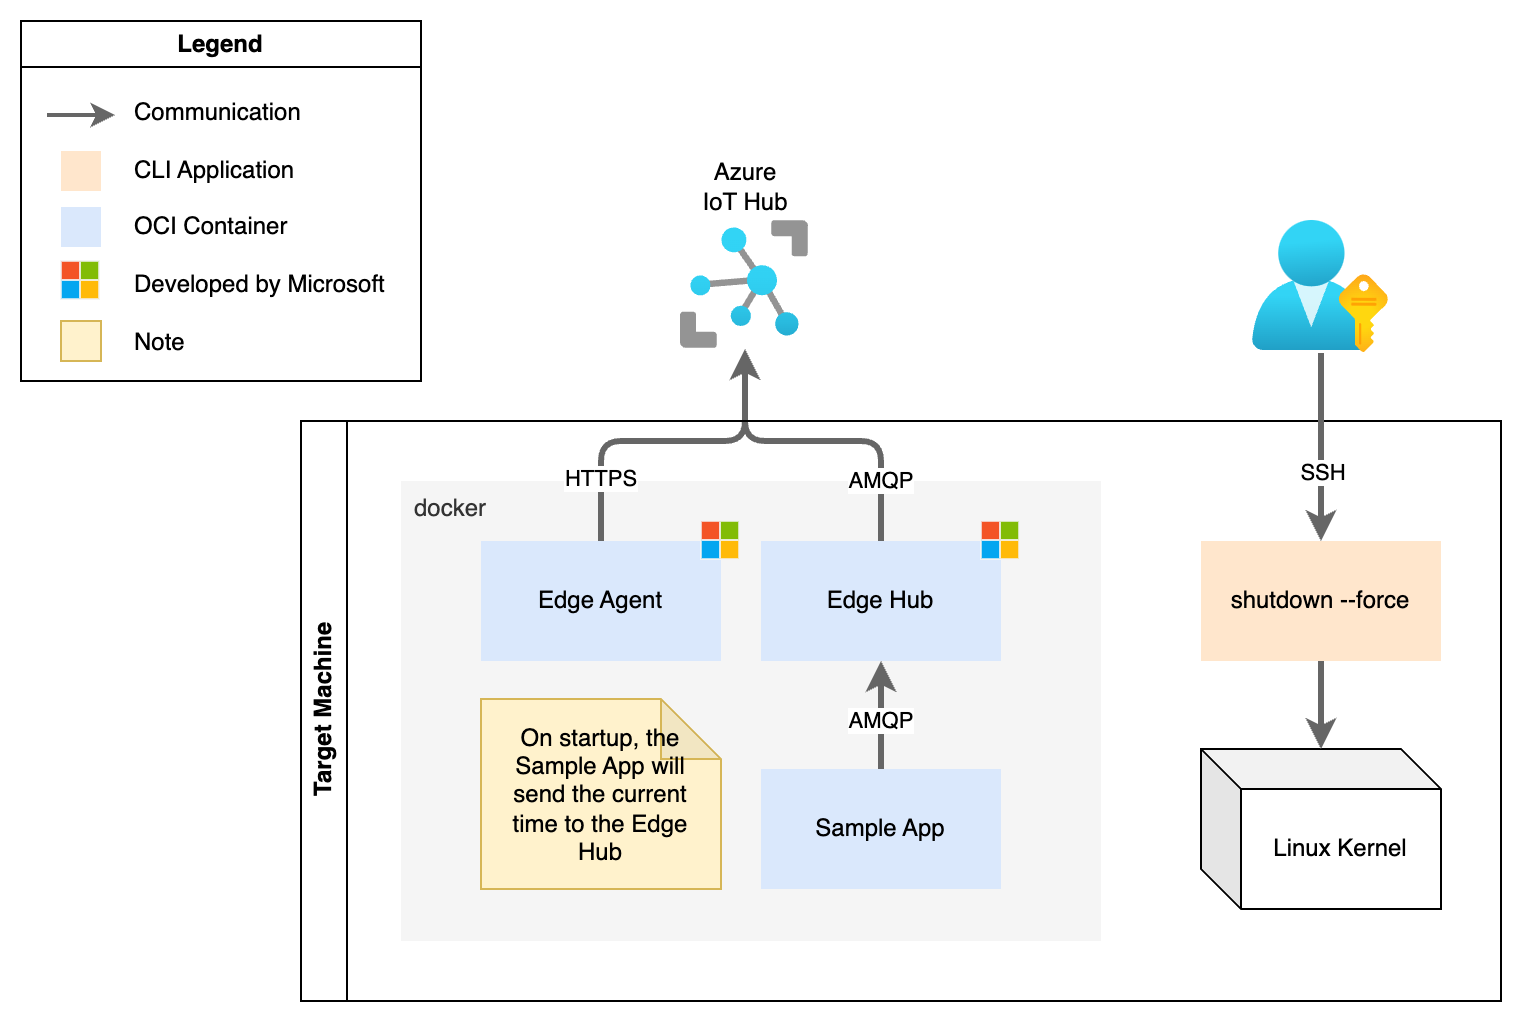
\includegraphics[width=0.75\textwidth]{fig/reboot-setup.drawio.png}
    \caption{Time To Recover Experiment Overview}
\end{figure}

\noindent
Just before the system is rebooted, the current time will be printed.
After the \ac{OS} rebooted and the Azure IoT Edge runtime has started, a
Sample App will send the current time to the Azure IoT Hub via the Azure IoT Edge
Hub, where it can be retrieved. The full shell command can be seen in listing
\ref{lst:reboot-command}.
\\

\begin{lstlisting}[
    caption=Command to print the current time and reboot,
    label=lst:reboot-command]
date +%s \
&& reboot -f
\end{lstlisting}

\noindent
When comparing the first timestamp ($t_0$) from the shell command output with the second
timestamp ($t_1$) from the \textit{Azure IoT Hub}, the time to recover can be calculated,
as the delta between those two timestamps:

\begin{equation}
    T := |t_1 - t_0|
\end{equation}
However, since rebooting the \ac{OS} is a process with many variances, the experiment
must be repeated multiple times. If we repeat the experiment $n$ times, where
$T_i$ represents the result of the $i$-th repetition, we can calculate
a mean value for $T$ as:

\begin{equation}
    \mu := \frac{\sum_{i=1}^{n}T_i}{n}
\end{equation}

\noindent
And the standard deviation for $T$ as:

\begin{equation}
   \sigma := \sqrt{\frac{\sum_{i=1}^{n}((T_i - \mu)^2}{n}}
\end{equation}

\noindent
Finally, the standard error for $T$ as:

\begin{equation}
    s := \frac{\sigma}{\sqrt{n}}
\end{equation}

\noindent
This experiment must be repeated, until the standard error is low enough
to have a confident mean value for each \ac{OS}.

\subsubsection{Hypothesis}
Our hypothesis is, that the time to recover will be very similar for all
\ac{OS}s, since the they all run \textit{Linux}, the Azure IoT Edge runtime and
a similar set of software, such as \textit{systemd} and \ac{SSH}. However, due
to the reduced size of \textit{reUpNix}, we may see a slight advantage in the
time to recover, since the \ac{OS} has to load less data from the disk. Further,
\textit{reUpNix} has a minified kernel and a reduced set of kernel modules.

\clearpage
\subsection{Container Updates}
When using Azure IoT Edge, \ac{IIoT} applications are deployed as containers, because
they change more frequent than the entire \ac{OS}. When a module is updated
with a new deployment manifest, Azure IoT Edge retrieves the any new container
images that are not present on the device. It uses a \ac{UDS} to communicate
with the container runtime, to pull the image. The same can be manually achieved
with the \code{docker pull} command, when using Docker as the container runtime.

\subsubsection{Setup}
\begin{enumerate}
    \item Obtain the container image (e.g. via \code{docker pull} or \code{docker build}),
    \item Fully unpack the image, including all layers,
    \item Merge all layers,
    \item Store the unpacked image in the Nix store,
    \item Include the Nix store object in to the system configuration,
    \item Load the image on boot.
\end{enumerate}
\subsubsection{Hypothesis}
Our hypothesis is, that updating containers with \textit{reUpNix}'s differential
update mechanism will be more efficient than updating them with Azure IoT Edge or
the \code{docker pull} command. This is due to the fact that, if the uppermost
layer of a container image, only contains minimal changes (e.g. only a few
changed files), the differential update will only transmit the changed files in
that layer, instead of the entire layer.


%\begin{tcolorbox}[title=TODO]
%Measurement results / analysis / discussion: 1/3
%\begin{itemize}
%\item whatever you have done, you must comment it, compare it to other systems, evaluate it
%\item usually, adequate graphs help to show the benefits of your approach
%\item caution: each result/graph must be discussed! what's the reason for this peak or why have you ovserved this effect
%\end{itemize}
%\end{tcolorbox}

\section{Image Size}
It has been possible to create a minimal \ac{OS} image with the Azure IoT Edge runtime
using \textit{reUpNix}. To achieve this, \textit{Nix} derivations and modules for
the \textit{Azure IoT Edge} runtime and the \textit{Azure IoT Edge Identity Service}
have been created. Additionally, a \textit{Nix} derivation for the \ac{ADU} Agent has been created.
Microsoft has the source code for the previously mentioned components
publicly available on GitHub, the \textit{Nix} packages could be built directly
from source, which is written in Rust and C and uses Cargo and CMake respectively.
For the third-party dependencies, namely \textit{libc}, \textit{libtss}, \textit{libcurl}, and
\textit{openssl}, of the \textit{Azure IoT Edge} runtime, the already existing \textit{Nix} packages
from the \textit{Nixpkgs} repository have been used.
By using the existing \textit{Nix} packages, it could be ensured that the dependencies
are linked with the correct paths in the \textit{Nix} store and can be reused
by other \textit{Nix} packages.
Further, the already existing \textit{Nix} package for \textit{Docker} had to be added
to the system configuration, since it is required by \textit{Azure IoT Edge}.
However, it is not a hard dependency, in case the user wants to exchange \textit{Docker}
with \textit{Moby} or \textit{Podman}, which are also able to run \ac{OCI}-compliant
container images.

Finally, since \textit{reUpNix} removes some unnecessary
Kernel modules, Kernel modules had to be added back to the system configuration in order
to be able to run \textit{Docker}.
Most notably, the kernel modules
\textit{br\_netfilter}, \textit{xt\_nat} and \textit{8021q} had to be added to the system configuration,
since they are required for \textit{Docker} networking.

\textit{reUpNix}, \textit{NixOS 23.01}, \textit{Ubuntu 22.04}, and
\textit{Yocto Kirkstone} had to be compared by their installed image size, with the methodology introduced
in chapter \ref{sec:image-size}. All system images feature an \ac{OCI}-compliant container runtime
and the Azure IoT Edge runtime. The results of the comparison are shown in table \ref{tab:image-size}.

\clearpage

\begin{table}[H]
	\centering
	\begin{tabular}{l|l|l}
	\toprule
		Operating System & Image Variation 1 & $\Delta$ Ubuntu\\
	\midrule
    \textbf{reUpNix} & \text{1 289 MB} & \color{ba-green}{- 1 010 MB} \\
    \textbf{NixOS 23.01} & \text{2 361 MB} & \textcolor{ba-red}{+ 62 MB} \\
    \textbf{Ubuntu 22.04} & \text{2 299 MB} & \text{-} \\
    \textbf{Yocto Kirkstone} & \text{4 933 MB} & \textcolor{ba-red}{+ 2 634 MB} \\
	\bottomrule
	\end{tabular}
	\caption{Image size by OS for each variation}
	\label{tab:image-size}
\end{table}

\noindent
It can be seen from table \ref{tab:image-size} that with its 1,289 \ac{MB},
\textit{reUpNix} has a 43\% smaller base image size than Microsoft's recommended
\textit{Ubuntu 22.04}. It is also 45\% smaller than the base image size of
\textit{NixOS 23.01}, which shows that the minification process is very effective
in minimizing the size of the \ac{OS} on disk despite having a fully working
Azure IoT Edge runtime installed.
To further illustrate the differences in size, refer to figure \ref{fig:image-size}.


\begin{figure}[htbp]
  \centering
  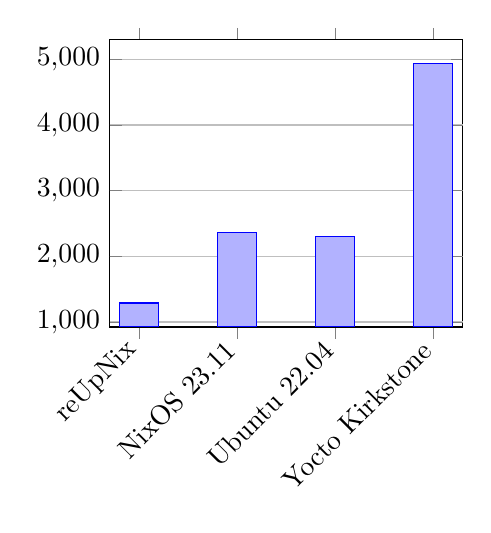
\begin{tikzpicture}
    \begin{axis}[
      ybar,
      bar width=0.5cm,
      width=0.5\textwidth,
      % height=0.5\textwidth,
      xtick=data,
      xticklabels={
        {reUpNix},
        {NixOS 23.11},
        {Ubuntu 22.04},
        {Yocto Kirkstone}
      },
      x tick label style={rotate=45,anchor=east}, % Rotating labels
      ymajorgrids=true, % Major grid lines for y-axis
      ytick={0,1000,2000,3000,4000,5000}, % Y-axis tick marks
      extra y ticks={1000,2000,3000,4000}, % Additional y-axis tick marks
      extra y tick labels={}, % Remove labels for the extra ticks
      ]

      \addplot coordinates {
        (1,1289)
        (2,2361)
        (3,2299)
        (4,4933)
      };

    \end{axis}
  \end{tikzpicture}
\caption{Image size by OS in Megabytes}
\label{fig:image-size}
\end{figure}

\noindent
In contrary, the difference in image size between \textit{Ubuntu 22.04} and
\textit{NixOS} is only 62 Megabytes, which is unsurprising, since both are
general purpose \textit{Linux} distributions and not specifically designed
for embedded and \ac{IoT} systems. The largest image in this comparison is
\textit{Yocto Kirkstone}, which is 2,634 Megabytes larger than \textit{Ubuntu 22.04}.
However, it features no effort to minimize the size of the \ac{OS} and it
just contains a default development configuration of the \textit{Yocto Project}
for \textit{Azure IoT Edge}. It can be seen that the hypothesis, that \textit{reUpNix}
is by far the smallest \ac{OS} in this comparison, is confirmed. The minification
process is effective and \textit{reUpNix} is a viable option for \ac{IoT} devices
running \textit{Azure IoT Edge} with limited storage capacity. Even if it would be
updated \textit{reUpNix} with an A/B partitioning scheme, which is not the proposed
methodology, the update size would be smaller, and it would still have less data
transmitted in comparison to the other \ac{OS}.

\subsection{Podman}
Podman is a container runtime developed by Red Hat and a direct competitor to Docker.
In the future it would be interesting to investigate the possibility of using
Podman instead of Docker as the container runtime for Azure IoT Edge. Podman is
not officially supported by Microsoft, but it can potentially be used as a
replacement for Docker, since it can provide a \ac{UDS} for the IoT Edge runtime
to communicate with the container runtime \cite{book:3556946,msdoc-supportetplatforms}.
In a quick comparison made with an unminified \textit{NixOS} image, it has been found that
using \textit{Podman} instead of \textit{Docker} would reduce the image size by
15\%. However, \textit{Podman} does not run on \textit{reUpNix} out of the box.
Some effort to investigate, which components have to be
added to \textit{reUpNix} be able to run \textit{Podman}, would have to be invested.

\section{Update size}
In the previous section it has already been discussed that it has been possible to create
\textit{Nix} packages for the \textit{Azure IoT Edge} runtime and its dependencies.
Since it has been established that \textit{reUpNix} can be used to create a minimal
\ac{OS} image for \textit{Azure IoT Edge}, the update size when updating with \textit{reUpNix}'s differential updates
can now be compared to the update size when updating in an A/B partitioning scheme.
Both methods can be used with \ac{ADU} Agent, with the exception that for \textit{reUpNix} the \ac{ADU}
needs to use a script handler to apply the update, while for A/B partitioning
the built-in \ac{ADU} handler can be used. When comparing the update size
for an update, which changes the majority of packages in the system, a \textit{Nixpkgs} version from November 1st, 2023 as the base and March 16th, 2024 as the target upstream have been picked. The results of the comparison are shown in table
\ref{tab:update-size}.

\begin{table}[H]
	\centering
	\begin{tabular}{l|l|l}
	\toprule
		Operating System & Image Variation 1 & $\Delta$ Ubuntu\\
	\midrule
    \textbf{reUpNix} & \text{206 MB} & \color{ba-green}{- 1 928 MB} \\
    \textbf{NixOS 23.01} & \text{XXXX MB} & \textcolor{ba-red}{+ XX MB} \\
    \textbf{Ubuntu 22.04} & \text{2 134 MB} & \text{-} \\
    \textbf{Yocto Kirkstone} & \text{4 717 MB} & \textcolor{ba-red}{+ 2 583 MB} \\
	\bottomrule
	\end{tabular}
	\caption{Update size by OS for each variation}
  \label{tab:update-size}
\end{table}

\noindent
It can be clearly seen that \textit{reUpNix} has a 90.3\% smaller update size
than \textit{Ubuntu 22.04}, which is a significant improvement. Applying the
differential update methodology of \textit{reUpNix} to \ac{IoT} devices
running \textit{Azure IoT Edge} will significantly reduce the amount of data
transmitted in comparison to using A/B partitioning. This is important for
devices with a limited Internet connection and it enables a more frequent updating.

\begin{figure}[htbp]
  \centering
  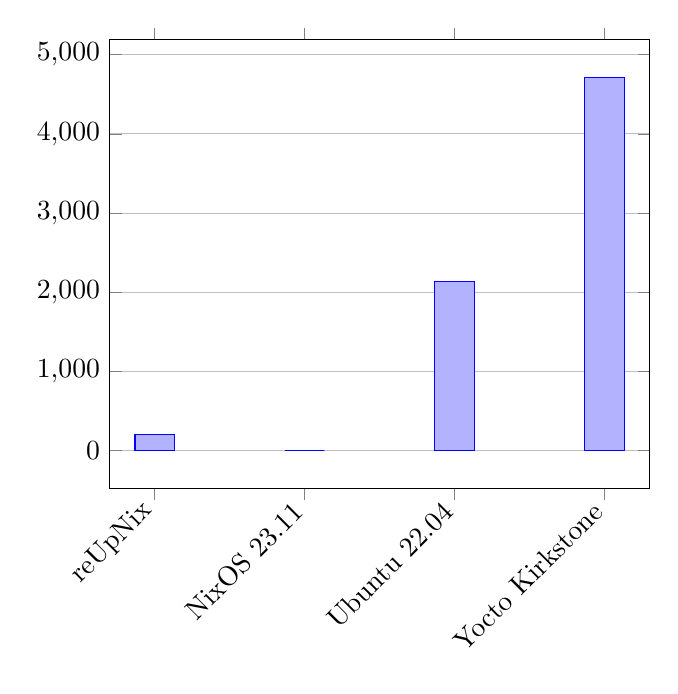
\begin{tikzpicture}
    \begin{axis}[
      ybar,
      bar width=0.5cm,
      % width=0.5\textwidth,
      % height=0.5\textwidth,
      xtick=data,
      xticklabels={
        {reUpNix},
        {NixOS 23.11},
        {Ubuntu 22.04},
        {Yocto Kirkstone}
      },
      x tick label style={rotate=45,anchor=east}, % Rotating labels
      ymajorgrids=true, % Major grid lines for y-axis
      ytick={0,1000,2000,3000,4000,5000}, % Y-axis tick marks
      extra y ticks={1000,2000,3000,4000}, % Additional y-axis tick marks
      extra y tick labels={}, % Remove labels for the extra ticks
      ]

      \addplot coordinates {
        (1,206)
        (2,0)
        (3,2134)
        (4,4717)
      };

    \end{axis}
  \end{tikzpicture}
\caption{Update Size by OS in Megabytes}
\label{fig:update-size}
\end{figure}

\noindent
In figure \ref{fig:update-size} it can be seen yet again how large the difference
in size is and that \textit{reUpNix} is the most efficient \ac{OS} in this comparison.
Using \textit{reUpNix} for \ac{IoT} devices running \textit{Azure IoT Edge}
instead of Microsoft's recommended \textit{Ubuntu 22.04} will significantly reduce
the data transmitted, when updating the \ac{OS} and the \textit{Azure IoT Edge} runtime.

\section{Time To Recover}
In order to verify that the \textit{reUpNix} system can recover from a reboot
in an acceptable time frame, the time it takes for the system to
reboot and send a message via the \textit{Azure IoT Edge Hub} with the proposed
methodology from chapter \ref{sec:time-to-recover} has been measured. The first message
that the \textit{Edge Agent} sends to the \textit{Edge Hub} after a reboot as
a measure has been used, because this message includes the timestamp when it was sent.
The \textit{Edge Agent} immediately sends an update message to the \textit{Azure
IoT Hub} to signal that the device is online. The same experiment has been repeated
for all of the \ac{OS}, namely \textit{reUpNix}, \textit{NixOS 23.01},
\textit{Ubuntu 22.04}, and \textit{Yocto Kirkstone}. The results of the comparison
can be seen in table \ref{tab:timetorecover} and figure \ref{fig:timetorecover}.


\begin{table}[H]
	\centering
	\begin{tabular}{l|l|l|l|l}
	\toprule
		Operating System & Average & Adjusted Average\footnote &  Std. Deviation & Std. Error \\
	\midrule
    \textbf{reUpNix} & 16.0 & 15.0 &  2.44 & 0.67 \\
    \textbf{NixOS 23.01} & 24.06 & 19.06 & 8.73 & 1.62 \\
    \textbf{Ubuntu 22.04} & 33.30 & 23.30 & 8.74 & 1.82 \\
    \textbf{Yocto Kirkstone} & 260.71 & 250.71 & 10.39  & 2.77 \\
	\bottomrule
	\end{tabular}
	\caption{Average Time to Recover by OS in Seconds}
	\label{tab:timetorecover}
\end{table}
\footnotetext{The adjusted average accounts for the delay that is configured in
the bootloader to wait for user input, which is 1 second for \textit{reUpNix},
5 seconds for \textit{NixOS 23.01}, and 10 seconds for \textit{Yocto Kirkstone}
and \textit{Ubuntu 22.04} respectively.}

\begin{figure}[H]
\centering
\begin{tikzpicture}
  \begin{axis}[
    title  = ReUpNix,
    ybar,
    bar width=0.05cm,
    enlarge y limits  = {0.15,upper},
    width = 0.3\textwidth,
  ]
    \addplot table [x=seconds, y=times, col sep=comma] {data/time-to-recover-reupnix.csv};
    \draw[dashed,red] (axis cs:15.33,\pgfkeysvalueof{/pgfplots/ymin}) -- (axis cs:15.33,\pgfkeysvalueof{/pgfplots/ymax});
    \draw[dashed] (axis cs:16,\pgfkeysvalueof{/pgfplots/ymin}) -- (axis cs:16,\pgfkeysvalueof{/pgfplots/ymax});
    \draw[dashed,red] (axis cs:16.67,\pgfkeysvalueof{/pgfplots/ymin}) -- (axis cs:16.67,\pgfkeysvalueof{/pgfplots/ymax});
  \end{axis}
\end{tikzpicture}
\begin{tikzpicture}
  \begin{axis}[
    title  = NixOS 23.01,
    ybar,
    bar width=0.05cm,
    enlarge y limits  = {0.15,upper},
    width = 0.3\textwidth,
    % nodes near coords,
  ]
    \addplot table [x=seconds, y=times, col sep=comma] {data/time-to-recover-nixos.csv};
    \draw[dashed,red] (axis cs:22.44,\pgfkeysvalueof{/pgfplots/ymin}) -- (axis cs:22.44,\pgfkeysvalueof{/pgfplots/ymax});
    \draw[dashed] (axis cs:24.06,\pgfkeysvalueof{/pgfplots/ymin}) -- (axis cs:24.06,\pgfkeysvalueof{/pgfplots/ymax});
    \draw[dashed,red] (axis cs:25.68,\pgfkeysvalueof{/pgfplots/ymin}) -- (axis cs:25.68,\pgfkeysvalueof{/pgfplots/ymax});
  \end{axis}
\end{tikzpicture}
\begin{tikzpicture}
  \begin{axis}[
    title  = Ubuntu 22.04,
    ybar,
    bar width=0.05cm,
    enlarge y limits  = {0.15,upper},
    width = 0.3\textwidth,
  ]
    \addplot table [x=seconds, y=times, col sep=comma] {data/time-to-recover-ubuntu.csv};

    \draw[dashed,red] (axis cs:31.48,\pgfkeysvalueof{/pgfplots/ymin}) -- (axis cs:31.48,\pgfkeysvalueof{/pgfplots/ymax});
    \draw[dashed] (axis cs:33.3,\pgfkeysvalueof{/pgfplots/ymin}) -- (axis cs:33.3,\pgfkeysvalueof{/pgfplots/ymax});
    \draw[dashed,red] (axis cs:35.12,\pgfkeysvalueof{/pgfplots/ymin}) -- (axis cs:35.12,\pgfkeysvalueof{/pgfplots/ymax});
  \end{axis}
\end{tikzpicture}
\begin{tikzpicture}
  \begin{axis}[
    title  = Yocto Kirkstone,
    ybar,
    enlarge y limits  = {0.15,upper},
    width = 0.3\textwidth,
    bar width=0.05cm,
  ]
    \addplot table [x=seconds, y=times, col sep=comma] {data/time-to-recover-yocto.csv};
    \draw[dashed,red] (axis cs:257.94,\pgfkeysvalueof{/pgfplots/ymin}) -- (axis cs:257.94,\pgfkeysvalueof{/pgfplots/ymax});
    \draw[dashed] (axis cs:260.71,\pgfkeysvalueof{/pgfplots/ymin}) -- (axis cs:260.71,\pgfkeysvalueof{/pgfplots/ymax});
    \draw[dashed,red] (axis cs:263.48,\pgfkeysvalueof{/pgfplots/ymin}) -- (axis cs:263.48,\pgfkeysvalueof{/pgfplots/ymax});
  \end{axis}
\end{tikzpicture}
\caption{Number of Measurements by Duration}
\label{fig:timetorecover}
\end{figure}
\noindent
It can be seen from the results that \textit{reUpNix} has on average the fastest time
to recover, from the four \ac{OS} that have been tested, even when accounting for the different
delays that are configured for the bootloader. So the hypothesis, that \textit{reUpNix}
and \textit{NixOS} will provide no significant delay in the boot process due to
the \textit{Nix} package manager, is confirmed. The two \ac{OS} using the
\textit{Nix} package manager have a similar or better, time to recover as the \ac{OS},
which use a traditional file system and directory structure, even when taking
the standard deviation and standard error into account. Some outliers
for \textit{Ubuntu 22.04} and \textit{NixOS 23.01} have been observed, which are due to the
fact that reboot command was issued without the force flag, which will cause
the system to wait until all processes are terminated before rebooting. Further,
it can be seen that \textit{reUpNix} has a faster time to recover than \textit{NixOS 23.01},
which means that the minification process of \textit{reUpNix} does not introduce
delay in the boot process and the opposite is true.
The measurements show that \textit{reUpNix} is a viable option for \ac{IoT} devices
and that the \textit{Nix} package manager does not introduce a significant delay.
\textit{Azure IoT Edge} with its dependencies can be installed and run on
\textit{reUpNix} with a comparable, even better, time to recover as Microsoft's
recommended \textit{Ubuntu 22.04}.


%\clearpage
\section{Container Installation}
With the proposed methodology in chapter \ref{sec:container-updates}, it has been possible
to install \ac{OCI}-container images on an \ac{IoT} device running \textit{reUpNix} without
using \code{docker pull}.
It has been verified that the installed images can be used to run containers with \textit{Docker}
and match the images from \textit{Docker Hub} by comparing the \textit{SHA256} checksums.
Since the images are now stored in the \textit{Nix} store, the \textit{reUpNix}
differential update mechanism has been used to install the container images and compare the update size
with the compressed size that would be downloaded with \code{docker pull}. In
contrast to \textit{Docker}, \textit{reUpNix} updates can be compressed with a
more efficient algorithm, since there's a freedom of choice up to the implementation.
\textit{Docker} uses \textit{gzip} for compressing images, while the updates with
\textit{reUpNix} in this comparison have been compressed with \textit{bzip2}.

Further, it was investigated if the update size can be further reduced by extracting
the file contents of the images layers into the \textit{Nix store}. This would mean
that \textit{Nix} can use file-level deduplication and \textit{reUpNix} can use
its differential update mechanism to reconstruct the files in the \textit{Nix store}
by using the already existing files on the device. The resulting update file was
then also compressed with \textit{bzip2}. However, due to the \textit{Nix store}
not preserving timestamps and order of files,
the reconstructed image does not have the same \textit{SHA256} checksum as the
original image from \textit{Docker Hub}, but the files are identical. For
\textit{Azure IoT Edge} this is not a problem, since the \textit{Edge Agent} only
references the image by its name and tag and not by its \textit{SHA256} checksum.


With this methodology the top 10 most pulled images from \textit{Docker Hub}
were examined and the results can be seen in table \ref{tab:container-size} and figure
\ref{fig:container-size}, where \textit{reUpNix (packed)} refers to the update
with its layers still being packed in a \textit{tar}-archive and \textit{reUpNix (unpacked)}
referring to the update with the layers being extracted and uncompressed into the
\textit{Nix store}.
\clearpage

\begin{figure}[htbp]
  \centering
  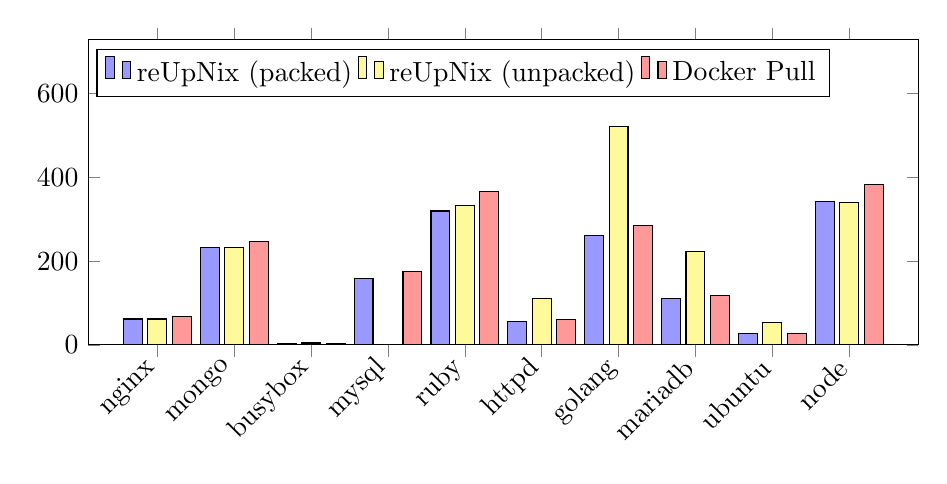
\begin{tikzpicture}
    \begin{axis}[
      ybar,
      width=1\textwidth,
      height=0.45\textwidth,
      enlarge y limits  = {0.4,upper},
      bar width=0.24cm,
      xtick=data,
      xticklabels={
        nginx, mongo, busybox, mysql, ruby, httpd, golang, mariadb, ubuntu, node
      },
      x tick label style={rotate=45,anchor=east},
      legend style={
        at={(0.01,0.97)},
        anchor=north west,
        legend columns=-1,
      }
      ]

      \addplot[fill=blue!40] coordinates {
        (1,61.83) % nginx
        (2,233.22) % mongo
        (3,2.03) % busybox
        (4,158.14) % mysql
        (5,319.78) % ruby
        (6,55.22) % httpd
        (7,261.24)  % golang
        (8,111.46) % mariadb
        (9,26.38) % ubuntu
        (10,343.49) % node
      };

      \addplot[fill=yellow!40] coordinates {
        (1,61.68) % nginx
        (2,233.41 ) % mongo
        (3,4.54) % busybox
        (4,0 ) % mysql
        (5,333.13 ) % ruby
        (6,110.75 ) % httpd
        (7,520.70 ) % golang
        (8,223.08 ) % mariadb
        (9,53.04 ) % ubuntu
        (10,340.26 ) % node
      };

      \addplot[fill=red!40] coordinates {
        (1,67.25) % nginx
        (2,246.58 ) % mongo
        (3,2.05) % busybox
        (4,174.94 ) % mysql
        (5,367.45 ) % ruby
        (6,61.53 ) % httpd
        (7,285.59 ) % golang
        (8,117.04 ) % mariadb
        (9,28.17 ) % ubuntu
        (10,382.26 ) % node
      };


      \legend{reUpNix (packed), reUpNix (unpacked), Docker Pull}
    \end{axis}
  \end{tikzpicture}
  \caption{Container Image Download Size in MB}
  \label{fig:container-size}
\end{figure}

\begin{table}[H]
	\centering
	\begin{tabular}{l|c|c|c|c|c}
	\toprule
	 Image & Docker Pull & reUpNix (Packed) & $\Delta$ \% & reUpNix (Unpacked) & $\Delta$ \%\\
	\midrule
    \textbf{nginx} & 67.25 MB & 61.83 MB & \color{ba-green}{- 8.0 \%} & 61.68 MB & \color{ba-green}{- 8.2 \%}\\
    \textbf{mongo} & 246.58 MB & 233.22 MB & \color{ba-green}{- 5.6 \%} & 233.41MB & \color{ba-green}{- 5.3 \%}\\
    \textbf{busybox} & 2.05 MB & 2.03 MB & \color{ba-green}{- 0.9 \%} & 4.54 MB & \color{ba-red}{+ 121.4 \%}\\
    \textbf{mysql} & 174.94 MB & 158.14 MB & \color{ba-green}{- 9.6 \%} & x & \color{ba-red}{+ x \%}\\
    \textbf{ruby} & 367.45 MB & 319.78 MB & \color{ba-green}{- 12.9 \%} & 333.13 MB & \color{ba-green}{- 9.3 \%}\\
    \textbf{httpd} & 61.53 MB & 55.22 MB & \color{ba-green}{- 10.2 \%} & 110.75 MB & \color{ba-red}{+ x \%}\\
    \textbf{golang} & 285.59 MB & 261.24 MB & \color{ba-green}{- 8.5 \%} & 520.70 MB & \color{ba-red}{+ x \%}\\
    \textbf{mariadb} & 117.04 MB & 111.46 MB & \color{ba-green}{- 4.7 \%} & 223.08 MB & \color{ba-red}{+ x \%}\\
    \textbf{ubuntu} & 28.17 MB & 26.38 MB & \color{ba-green}{- 6.3 \%} & 53.04 MB & \color{ba-red}{+ 84.7 \%}\\
    \textbf{node} & 382.26 MB & 343.49 MB & \color{ba-green}{- 10.1 \%} & 340.26MB & \color{ba-green}{- 10.9 \%}\\
	\bottomrule
	\end{tabular}
	\caption{Container Image Download Size}
	\label{tab:container-size}
\end{table}

\noindent
It can been seen from the results, that the \textit{reUpNix} differential update mechanism
with the image layers still being packed in a \textit{tar}-archive is more efficient
in installing container image updates, than using \code{docker pull}.
However, this is mostly due to the fact that the updates are compressed with \textit{bzip2}
instead of \textit{gzip}. A quick check when compressing the update with \textit{gzip}
showed that the sizes are almost identical to the sizes of the images downloaded
with \code{docker pull}.
For all of the top 10 most pulled images from \textit{Docker Hub}, we can save
transferred data size by using \textit{reUpNix} and \textit{bzip2}. This means
that using \textit{reUpNix} to install container images on \ac{IoT} devices is more
efficient than using \code{docker pull} and the proposed methodology can be used
as a replacement which still works with \textit{Azure IoT Edge}.

For using the \textit{reUpNix} differential update mechanism to install container
with the layers of the image being extracted and uncompressed into the
\textit{Nix store}, we can see that the update size is also smaller
than the size of the \code{docker pull} command, when using \textit{bzip2} to
compress the entire update. For some images, there is a slight advantage in size
when
unpacking the layers. This is mostly due to the fact that the layers
contain files than can be recreated from existing files on the device.

The hypothesis proposed in this thesis, that the \textit{reUpNix} differential
update mechanism can be used to install container images on \ac{IoT} devices
running \textit{Azure IoT Edge} was shown to be true and the results show that
using \textit{reUpNix} will save data transmitted when installing container images.


\section{Container Updates}
For \ac{IoT} devices running \textit{Azure IoT Edge}, installing new containers
is not the only use case. In most scenarios, existing containers will be updated
with a newer version to include new features or security patches. It was already
shown in the previous section that the \textit{reUpNix} differential update mechanism
can be used to install container images on \ac{IoT} devices running \textit{Azure IoT Edge}.
To measure the efficiency of the \textit{reUpNix} differential update mechanism
when updating container images, a selection of the most popular container images
from \textit{Docker hub} were updated to the latest version from the previous version
using the \textit{reUpNix} differential update mechanism. \textit{Docker} uses
\textit{gzip} to compress the layers of the image when pulling. For the differential
updates of \textit{reUPNix}, \textit{gzip} was also used to compress the updates,
however, the update can be compressed with any algorithm. The results of the
comparison can be seen in table \ref{tab:container-update-size}.

\begin{table}[H]
	\centering
  \footnotesize
	\begin{tabular}{l|c|c|c|c|c|c}
	\toprule
	 Image & From& To & Layers & Pull Size & reUpNix Size &$\Delta$ \% \\
	\midrule
    \textbf{ubuntu} & jammy-20240212 & jammy-20240227 & 1 & 29.54 MB &28.72 MB & \color{ba-green}{- 2.77 \%} \\
    \textbf{node} & 20.12.0-bullseye & 21.7.1-bullseye & 13 & 357.03 MB & 362.64 MB & \color{ba-red}{+ 1.57 \%} \\
    \textbf{ruby} & 3.1.4-bookworm & 3.2.3-bookworm & 16 & 365.76 MB & 372.82 MB & \color{ba-red}{+ 1.93 \%} \\
    \textbf{busybox} & 1.35.0-glibc & 1.36.1-glibc & 1 & 2.05 MB & 2.15 MB & \color{ba-red}{+ 4.87 \%} \\
	\bottomrule
	\end{tabular}
	\caption{Container Image Update Size}
	\label{tab:container-update-size}
\end{table}

\noindent
The results show that when using the \textit{reUpNix} differential update mechanism
to update container images, the size of the update is slightly larger than the size
when using \code{docker pull} for most of the tested images. This is mostly due
to the fact that when vendors
publish new versions of their container images, they usually include new features
and update the software in the image, which means that almost all files on all
layers have to be updated.

The additional size can be explained by the fact that the \textit{reUpNix}
differential update mechanism takes up some space for the update script itself,
which needs to store information about \textit{Nix store} paths were the files
to update are located.

The established hypothesis, that the \textit{reUpNix} differential update mechanism
are more efficient than using \code{docker pull} for updating container images
is not true. There are however images, like \textit{ubuntu}, where the update size
was smaller when updating with \textit{reUpNix}, but this was mainly due to the
fact that the time between releases was the shortest for this image.

\subsection{Improved Compression}
To further reduce the update size, the \textit{reUpNix} differential updates can
be compressed with a more efficient algorithm than \textit{gzip}. With \textit{reUpNix}
updates, users are not bound to \textit{gzip}, like with docker. A quick test
yielded that using \textit{bzip2} to compress the updates instead of \textit{gzip},
the update size can be further reduced. For example, the container image \textit{ubuntu}
was 6.3\% smaller when compressed with \textit{bzip2} instead of \textit{gzip}.


\section{Summary}
\begin{tcolorbox}[title=TODO]
Summarize again what the paper did, but now emphasize more the results, and comparisons
\end{tcolorbox}

\section{Conclusion}
This section will highlight the main findings of the thesis to provide a
conclusion, so that \ac{IIoT} application developers and product managers can
make a careful consideration when choosing an \ac{OS} for their \ac{IIoT} devices.

\subsection{Image And Update Size}
It was shown that reUpNix has the the potential to drastically reduce the transferred
data when updating the operating system, which is important for \ac{IIoT} devices
that have a limited Internet connection.

\subsection{Updating Docker Containers}

\begin{tcolorbox}[title=TODO]
    Highlight how updating Docker containers with reUpNix is more efficient than
    updating them with \code{docker pull}.
\end{tcolorbox}

\subsection{Limited Microsoft Support}
Microsoft does not officially support NixOS or reUpNix, which may be a decisive factor
for product managers choosing an \ac{OS} for their \ac{IIoT} devices. Microsoft
only provides so called "Tier 1" support for Ubuntu, Debian, Red Hat Enterprise
Linux and Windows, which means that Microsoft is actively testing and validating
new releases. If a developer is using an \ac{OS} that is not officially supported
and encounters a problem, they need to reproduce the issue with one of Microsoft's
"Tier 1" supported \ac{OS} before they can open a support ticket with Microsoft
\cite{msdoc-supportetplatforms}.

\section{Future Work}

\subsection{Podman}
Podman is a container runtime developed by Red Hat and a direct competitor to Docker.
In the future it would be interesting to investigate the possibility of using
Podman instead of Docker as the container runtime for Azure IoT Edge. Podman is
not officially supported by Microsoft, but it can potentially be used as a
replacement for Docker, since it can provide a \ac{UDS} for the IoT Edge runtime
to communicate with the container runtime \cite{book:3556946,msdoc-supportetplatforms}.

\subsection{Implementing A Update Agent Handler}
\begin{tcolorbox}[title=TODO]
Microsoft allows to implement their own update agent handler, which could be
used to implement a custom update agent handler that is compatible with reUpNix.
\end{tcolorbox}

\subsection{Further minification}
\begin{tcolorbox}[title=TODO]
Elaborate that this thesis has NOT shown the absolute smallest possible system
to run Azure IoT Edge on, and that there's still room for further minification.
\begin{itemize}
    \item Minify Microsoft's software e.g. by compiling with \code{-w} and \code{-s} flags
    \item Or using software like \textit{upx} to compress binaries
    \item Minify Podman and/or Docker runtime
\end{itemize}
\end{tcolorbox}

\subsection{Code optimization}
As with most software projects, the written source code for this thesis could
almost always be optimized to be written to run faster, use less resources, be
more concise and be more readable. As the knowledge about the system and the
Nix language grows, and the helper functions added to Nix increase, the
written configuration files can be optimized. At the time of the research, the
Nix build process takes a lot of time and resources, and an optimization could
lead to an increase in productivity and less time spent waiting.


\cleardoublepage

\pagestyle{fancy-lists}

% \phantomsection is needed for hyperref to reference the correct
% page.

\phantomsection
% special page style for the unnumbered lists chapter and its sections.  This
% prevents numbers in the headers.  The title is set via \chaptermark and
% \sectionmark, see below.
\addcontentsline{toc}{chapter}{\listoftitlename}%
\chaptermark{\listoftitlename}

\addcontentsline{toc}{section}{\glossarytitlename}%
\sectionmark{\glossarytitlename}
\chapter*{\glossarytitlename}

\begin{acronym}
\acro{OS}{Operating System}
\acro{IoT}{Internet of Things}
\acro{IIoT}{Industrial IoT}
\acro{OCI}{Open Container Initiative}
\acro{SDK}{Software Development Kit}
\acro{OTA}{Over The Air}
\acro{API}{Application Programming Interface}
\acro{REST}{Representational State Transfer}
\acro{HTTP}{Hypertext Transfer Protocol}
\end{acronym}

\cleardoublepage

\phantomsection
\addcontentsline{toc}{section}{\listfigurename}%
\sectionmark{\listfigurename}
\listoffigures
\cleardoublepage

\phantomsection
\addcontentsline{toc}{section}{\listtablename}%
\sectionmark{\listtablename}
\listoftables
\cleardoublepage

\phantomsection
\addcontentsline{toc}{section}{\listlistingname}%
\sectionmark{\listlistingname}
\listoflistings
\cleardoublepage

\phantomsection
\addcontentsline{toc}{section}{\listalgorithmname}%
\sectionmark{\listalgorithmname}
\listofalgorithms
\cleardoublepage

\phantomsection
\addcontentsline{toc}{section}{\bibname}%
\sectionmark{\bibname}
\printbibliography

\end{document}
